\documentclass[12pt]{article}
\usepackage{geometry}
\usepackage{graphicx} % 插图
\usepackage{float} % 插图位置固定
\usepackage{amsmath} % 文字加粗
\usepackage[UTF8]{ctex} %中文宏包
\setCJKmainfont{SimSun}
\usepackage{fontspec} %引入字体设置宏包
\setmainfont{Times New Roman}
\usepackage{indentfirst} %首行缩进
\usepackage{listings} %代码
\usepackage{color} %字体颜色
\usepackage{subfigure}  %插入多图时用子图显示的宏包

\usepackage{minted} %代码
\usemintedstyle{vs}


%\usepackage{fancyhdr} %页眉页脚
%\pagestyle{fancy} 
%\fancyhf{}
%\lhead{数字图像处理}
%\chead{Noise Reduction Using a Median Filter}
%\rhead{张青铭 \quad 3200105426}
%\renewcommand{\headrulewidth}{0pt}
%图片路径
\graphicspath{ {figures/} }

%页面格式
\geometry{a4paper,
left=20mm,
right=20mm,
top=20mm,
bottom=20mm }

\title{{\Huge{\textbf{数字图像处理}}}\\Pro11-1\quad  Boundary following}
\author{信息与电子工程学院\quad 信息工程 \quad 3200105426\\张青铭}
\date{\today}

\begin{document}
\maketitle
\section{实验任务}
(1)实现边界跟随算法,确保输出边界中的点按顺时针或逆时针顺序组织;

(2)下载图9.14,用设计的算法得到其边界;
\section{算法设计}
算法步骤:

1.遍历图像;

2.标记第一个遇见像素块的前景像素$(i,j)$;

3.对这个像素周围八邻域逆时针搜索,如果搜索到周围有前景像素,那么更新坐标$(i,j)$为$(i',j')$,并标记;

4.不断执行第3步直到再次遇见此像素块第一次标记的像素;

5.继续执行第1步;

\section{代码实现}
\begin{minted}[frame=lines,tabsize=4,python3,baselinestretch=0.85]{matlab}
clear all;
close all;
clc;

img=imread('fig.tif');
[m n]=size(img);

imgn=zeros(m,n);        %边界标记图像
ed=[-1 -1;0 -1;1 -1;1 0;1 1;0 1;-1 1;-1 0]; %从左上角像素,逆时针搜索
for i=2:m-1
for j=2:n-1
    if img(i,j)==1 && imgn(i,j)==0      %当前是没标记的白色像素
        if sum(sum(img(i-1:i+1,j-1:j+1)))~=9    %块内部的白像素不标记
            ii=i;         %像素块内部搜寻使用的坐标
            jj=j;
            imgn(i,j)=2;    %本像素块第一个标记的边界,第一个边界像素为2
            
            while imgn(ii,jj)~=2    %是否沿着像素块搜寻一圈了。
                for k=1:8           %逆时针八邻域搜索
                    tmpi=ii+ed(k,1);        %八邻域临时坐标
                    tmpj=jj+ed(k,2);
                    if img(tmpi,tmpj)==1 && imgn(tmpi,tmpj)~=2  %搜索到新边界,并且没有搜索一圈
                        ii=tmpi;        %更新内部搜寻坐标,继续搜索
                        jj=tmpj;
                        imgn(ii,jj)=1;  %边界标记图像该像素标记,普通边界为1
                        break;
                    end
                end
            end
            
        end
    end
end
end
figure;
imgn=imgn>=1;
subplot(1,2,2);imshow(imgn,[]);title('边界')
subplot(1,2,1);imshow(img);title('原图')
\end{minted}

\section{实验结果}
将算法应用与图9.14得到结果如下:
\begin{figure}[H]
	\centering
	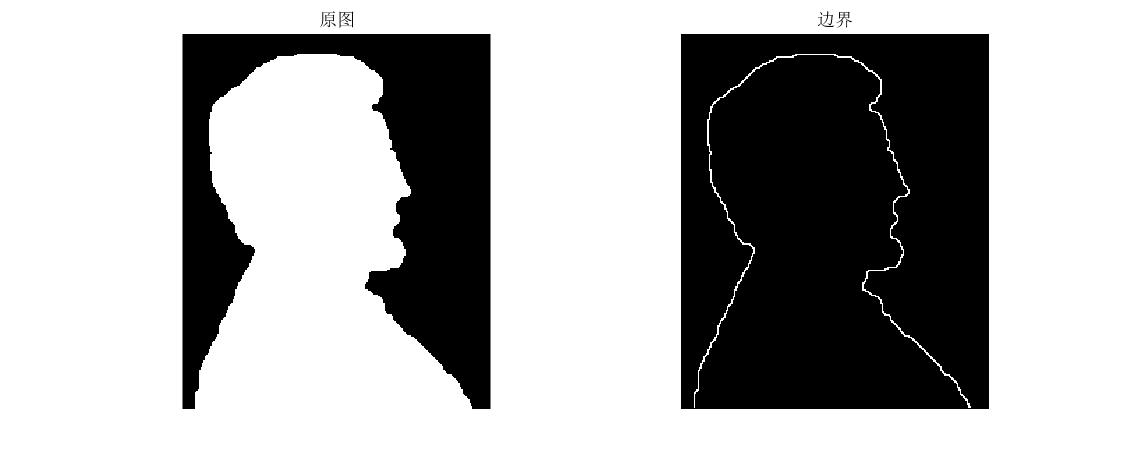
\includegraphics[width=0.8\linewidth]{figures/fig}
	\caption{边界跟踪}
\end{figure}

\section{总结}
本次实验实现了一个边界跟踪算法,其本质就是不断对目标像素做八邻域遍历的迭代算法,最终的实现效果也比较不错。
\end{document}
